\documentclass[a4paper]{article}
\usepackage[14pt]{extsizes} 
\usepackage[T2A]{fontenc}
\usepackage[utf8]{inputenc}
\usepackage{natbib}
\usepackage{graphicx}
\usepackage{amsmath}
\usepackage[english, russian]{babel}
\usepackage{amsmath,amsfonts,amssymb,amsthm,mathtools,mathrsfs}
\usepackage{icomma}
\usepackage{fullpage}
\usepackage{ulem}
\usepackage{eufrak}
\usepackage{setspace}
\usepackage{listings}
\usepackage{indentfirst}
\usepackage[left=2cm,right=1.5cm,top=2cm,bottom=2cm]{geometry}
\usepackage{xcolor}
\usepackage{float}
\usepackage{csquotes}

\setlength{\parindent}{5ex}
\setlength{\parskip}{1em}
\renewcommand{\baselinestretch}{1}

\graphicspath{{images/}}

\definecolor{buzzlightyear}{HTML}{8757A5}
\definecolor{grass}{HTML}{738D06}
\definecolor{literal}{HTML}{F18A2B}
\definecolor{commentcolor}{HTML}{8E908B}

\lstdefinestyle{habrstyle}{
    backgroundcolor=\color{white},   
    commentstyle=\color{commentcolor},
    keywordstyle=\bfseries\color{buzzlightyear},
    numberstyle=\tiny\color{commentcolor},
    stringstyle=\color{grass},
    basicstyle=\ttfamily\footnotesize,
    breakatwhitespace=false,         
    breaklines=true,                 
    captionpos=b,                    
    keepspaces=true,                 
    numbers=left,                    
    numbersep=5pt,                  
    showspaces=false,                
    showstringspaces=false,
    showtabs=false,                  
    tabsize=4
}

\lstset{style=habrstyle}

\begin{document}
    % НАЧАЛО ТИТУЛЬНОГО ЛИСТА
    \begin{center}
        \begin{center}
        \hfill \break
        \normalsize{Санкт-Петербургский государственный политехнический}\\
        \normalsize{университет Петра Великого}\\
        \hfill \break
        \normalsize{\textbf{Высшая школа интеллектуальных систем и}}\\ 
        \normalsize{\textbf{суперкомпьютерных технологий}}\\ 
        \hfill \break
        \hfill \break
        \hfill \break
        \normalsize{Лабораторная работа №6}\\
        \hfill \break
        \hfill \break
        \normalsize{\LARGE Дискретное косинусное преобразование}\\
        \end{center}
        \hfill \break
        \hfill \break
        \hfill \break
        \hfill \break
        \hfill \break
        \hfill \break
        \hfill \break
        \hfill \break
        \hfill \break
        \hfill \break
        \begin{flushright}
            \normalsize{Выполнил студент 3-го курса}\\
            \normalsize{группа 3530901/80201}\\
            \normalsize{Матвеец Андрей Вадимович}\\
            \hfill \break
            \normalsize{Преподаватель:}\\
            \normalsize{Богач Наталья Владимировна}\\
        \end{flushright}
        \hfill \break
        \hfill \break
        \hfill \break
        \hfill \break
        \begin{center} Санкт-Петербург\end{center}
        \begin{center}2021\end{center} 
        \thispagestyle{empty}
    \end{center}
    % КОНЕЦ ТИТУЛЬНОГО ЛИСТА
    
    % ОГЛАВЛЕНИЕ
    \newpage
        \tableofcontents
    
    % СПИСОК ИЛЛЮСТРАЦИЙ
    \newpage
         \listoffigures
    
    % СПИСОК ЛИСТИНГОВ     
    \newpage
         \lstlistoflistings   
     
    \newpage
        \section{Часть №1: \texttt{timeint}}
            В первой части  лабораторной работы нам необходимо проверить тот факт, что \texttt{analyze1} требует времени пропорционально $n^2$, а \texttt{analyze2} пропорционально $n^3$ путем запуска их с несколькими разными массивами. Для этого необходимо воспользоваться \texttt{timeint}
            
            Для этого сначала создадим сигнал на основе некоррелируемом гауссовском шуме:
            
            \begin{figure}[H]
                \centering
                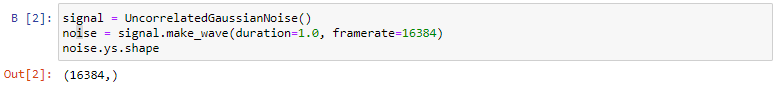
\includegraphics[width=\textwidth]{ex_1_UGN_signal.png}
                \caption{Создание сигнала}
                \label{fig:ex_1_UGN_signal}
            \end{figure}
            
            Далее создаем массив с тестовыми данными:
            
            \begin{figure}[H]
                \centering
                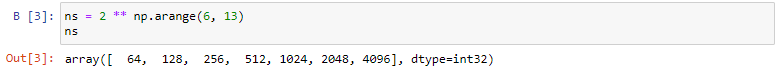
\includegraphics[width=\textwidth]{ex_1_UGN_array.png}
                \caption{Создание массива}
                \label{fig:ex_1_UGN_array}
            \end{figure}
            
            Теперь создадим функцию, которая будет стоить результаты и рисовать прямую линию из массива результатов из временного эксперимента:
            
\begin{lstlisting}[language=Python, caption= Функция \texttt{plot-bests}]
    def plot_bests(bests):    
        thinkplot.plot(ns, bests)
        thinkplot.config(xscale='log', yscale='log', legend=False)
        
        x = np.log(ns)
        y = np.log(bests)
        t = linregress(x,y)
        slope = t[0]
    
        return slope
\end{lstlisting}
            
            Сразу после этого создаем функцию \texttt{analyze1}
            
\begin{lstlisting}[language=Python, caption= Функция \texttt{analyze1}]
    def analyze1(ys, fs, ts):
        args = np.outer(ts, fs)
        M = np.cos(PI2 * args)
        amps = np.linalg.solve(M, ys)
        return amps
\end{lstlisting}
            
            Протестируем данную функцию и посмотрим получившиеся пезультаты:
            
            \begin{figure}[H]
                \centering
                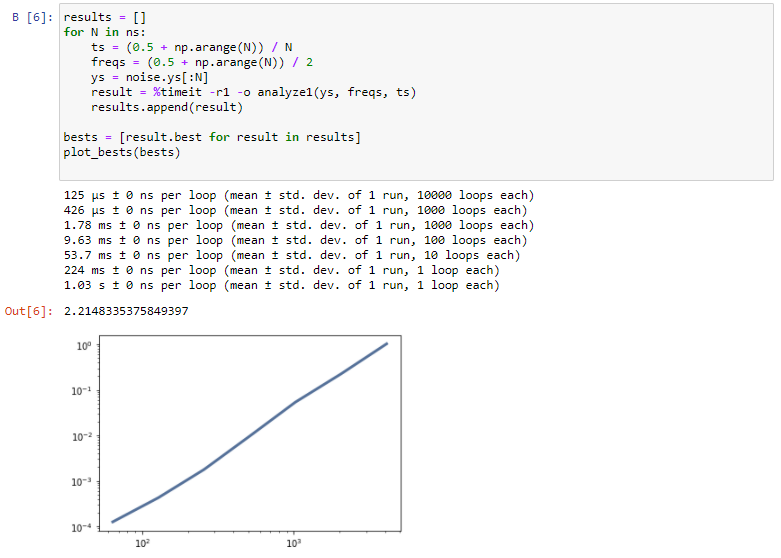
\includegraphics[width=\textwidth]{ex_1_analyze1_result.png}
                \caption{Тестирование \texttt{analyze1}}
                \label{fig:ex_1_analyze1_result}
            \end{figure}
            
            Теперь создадим функцию \texttt{analyze2}
            
\begin{lstlisting}[language=Python, caption= Функция \texttt{analyze2}]
    def analyze2(ys, fs, ts):
        args = np.outer(ts, fs)
        M = np.cos(PI2 * args)
        amps = np.dot(M, ys) / 2
        return amps
\end{lstlisting}
            
            И также протестируем ее:
            
             \begin{figure}[H]
                \centering
                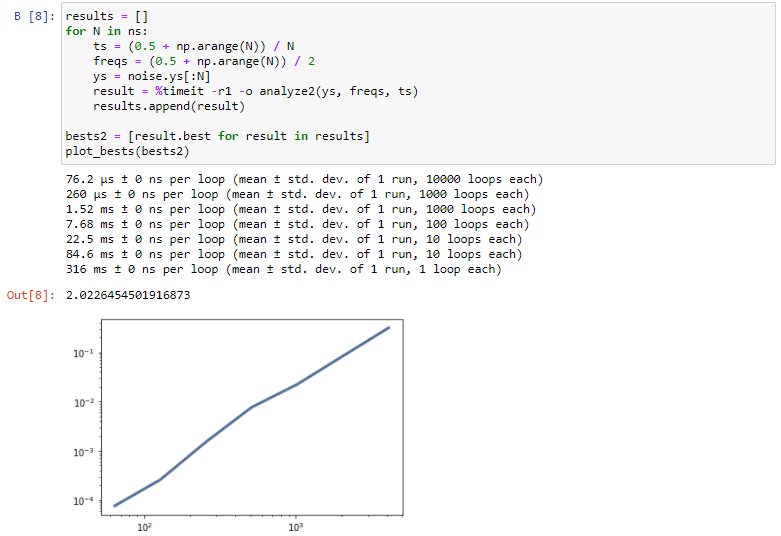
\includegraphics[width=\textwidth]{ex_1_analyze2_result.png}
                \caption{Тестирование \texttt{analyze2}}
                \label{fig:ex_1_analyze2_result}
            \end{figure}
            
            Для более удобного сравнения отобразим оба графика на одном поле:
            
\begin{lstlisting}[language=Python, caption= Сравнение результатов]
    thinkplot.plot(ns, bests, label='analyze1')
    thinkplot.plot(ns, bests2, label='analyze2')
    decorate(xlabel='Wave length (N)', ylabel='Time (s)', **dict(xscale='log', yscale='log'))
\end{lstlisting}               
            
            \begin{figure}[H]
                \centering
                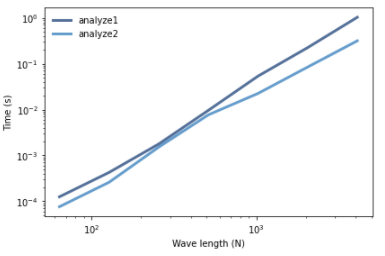
\includegraphics{ex_1_comparison .png}
                \caption{Сравнение результатов}
                \label{fig:ex_1_comparison}
            \end{figure}
            
            В результате можно сделать вывод, что \texttt{analyze2} работает быстрее, чем \\ \texttt{analyze1}
    
    \newpage
        \section{Часть №2: Реализация алгоритма сжатия звука}
            Во втором пункте лабораторной работы нам необходимо реализовать версию ДКП алгоритма для сжатия звука.
            
            Начнем с того, что скачаем звук сирены при воздушной атаке:
            
             \begin{figure}[H]
                \centering
                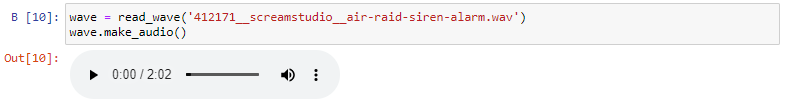
\includegraphics[width=\textwidth]{ex_2_audio.png}
                \caption{Получение звука}
                \label{fig:ex_2_audio}
            \end{figure}
            
            Далее нам необходимо выделить некоторый сегмент. Был выбрал сегмент с 5 секунды длительностью 0,5 секунды:
            
            \begin{figure}[H]
                \centering
                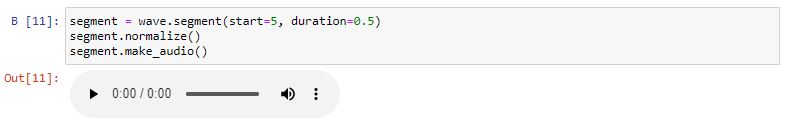
\includegraphics[width=\textwidth]{ex_2_segment.png}
                \caption{Получение сегмента}
                \label{fig:ex_2_segment}
            \end{figure}
            
            После этого выведем график амплитуды нашего сегмента:
            
\begin{lstlisting}[language=Python, caption= Полученние графика амплитуды сегмента]
    seg_dct = segment.make_dct()
    seg_dct.plot(high=4000)
    decorate(xlabel='Frequency (Hz)', ylabel='DCT')
\end{lstlisting}               
            
            \begin{figure}[H]
                \centering
                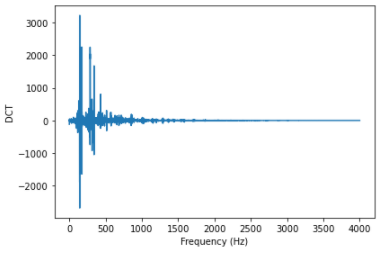
\includegraphics{ex_2_segment_dct.png} 
                \caption{Полученный график амплитуды сегмента}
                \label{fig:ex_2_segment_dct}
            \end{figure}
            
            По графику видно, что в сегменте очень много точек с нулевой амплитудой. Напишем функцию \texttt{compress} для зануления элементов, которые ниже порога \texttt{thres}:
            
\begin{lstlisting}[language=Python, caption= Функция \texttt{compress}]
    def compress(dct, thresh=1):
        count = 0
        for i, amp in enumerate(dct.amps):
            if np.abs(amp) < thresh:
                dct.hs[i] = 0
                count += 1
                
        n = len(dct.amps)
        print(count, n, 100 * count / n, sep='\t')
\end{lstlisting}      
            
            Применим написанную функцию к нашему сегменту:
            
\begin{lstlisting}[language=Python, caption= Применение функции \texttt{compress} к сегменту]
    seg_dct = segment.make_dct()
    compress(seg_dct, thresh=10)
    seg_dct.plot(high=4000)
\end{lstlisting}               
            
            \begin{figure}[H]
                \centering
                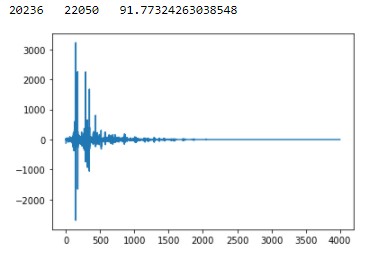
\includegraphics{ex_2_segment_dct_compress.png} 
                \caption{Результат применения функции \texttt{compress} к сегменту}
                \label{fig:ex_2_segment_dct_compress}
            \end{figure}
            
            Визуально графики ничем не отличаются друг от друга. 
            
            Ради интереса создадим аудиодорожку из полученного сегмента после \\ \texttt{compress}:
            
            \begin{figure}[H]
                \centering
                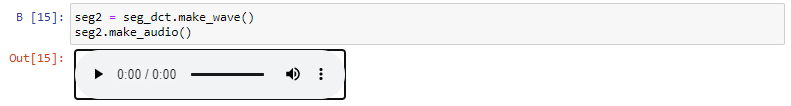
\includegraphics[width=\textwidth]{ex_2_segment_dct_compress_audio.png}
                \caption{Получение сегмента}
                \label{fig:ex_2_segment_dct_compress_audio}
            \end{figure}
            
            При прослушивании и сравнение полученной аудиодорожки с оригинальной можно сделать вывод, что, как мне показалось, появились некоторые шумы.
            
            Чтобы сжать более длинный фрагмент нам необходимо написать класс, который будет делать спектограмму ДКП :
            
\begin{lstlisting}[language=Python, caption= Класс \texttt{make-dct-spectrogram}]
    def make_dct_spectrogram(wave, seg_length):
        window = np.hamming(seg_length)
        i, j = 0, seg_length
        step = seg_length // 2
        spec_map = {}
    
        while j < len(wave.ys):
            segment = wave.slice(i, j)
            segment.window(window)
    
            t = (segment.start + segment.end) / 2
            spec_map[t] = segment.make_dct()
    
            i += step
            j += step
    
        return Spectrogram(spec_map, seg_length)
\end{lstlisting} 
            
            Теперь нам необходимо создать спектограмму ДКП и применить функцию \texttt{compress} к каждому сегменту:
            
            \begin{figure}[H]
                \centering
                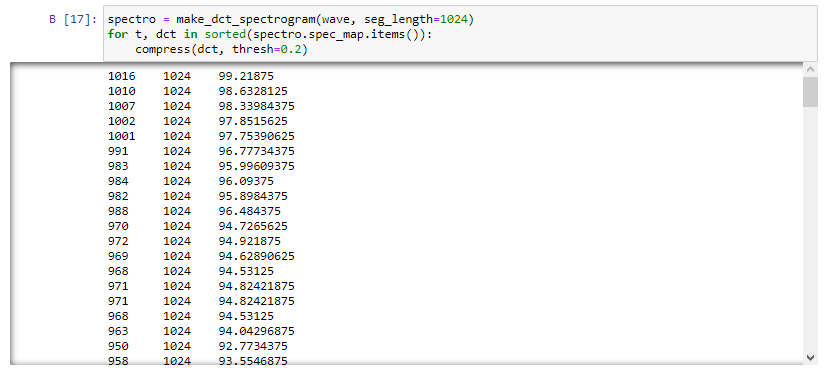
\includegraphics[width=\textwidth]{ex_2_spectogramma.png}
                \caption{Получение спектограммы для всех сегментов сигнала}
                \label{fig:ex_2_spectogramma}
            \end{figure}
            
            Так как вывелось огромное количество сегментов, я привел в пример только часть из них. Все результаты можно увидеть в файле \texttt{lab6.ipynb}. 
            
            Наконец, переведем полученную спектограмму в сигнал, чтобы сравнить ее с исходным сигналом:
            
            \begin{figure}[H]
                \centering
                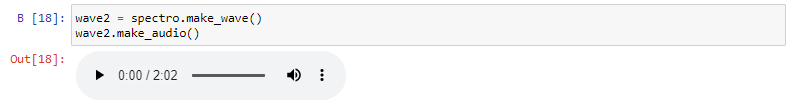
\includegraphics[width=\textwidth]{ex_2_result_audio.png}
                \caption{Получение спектограммы для всех сегментов сигнала}
                \label{fig:ex_2_result_audio}
            \end{figure}
            
            При прослушивании исходного сигнала и полученного в результате, можно сделать вывод, что после всех манипуляций в сигнале появился шум, которым можно управлять с помошью взаимодействия с порогом \texttt{thres}.
            
    \newpage
        \section{Часть №3: \texttt{phase.ipynb}}
            В третьем пункте шестой лабораторной работы нам необходимо запустить блокнот \texttt{phase.ipynb}, пройтись по всем примерам, после чего выбрать любой другой сегмент и сделать с ним те же самые манипуляции.
            
            В блокноте \texttt{phase.ipynb} содержится функция \texttt{plot-angle}, которая отображает амплитуды, форму волны и \texttt{angle} для спектра:
            
\begin{lstlisting}[language=Python, caption= Функция \texttt{plot-angle}]
    def plot_angle(spectrum, thresh=1):
        angles = spectrum.angles
        angles[spectrum.amps < thresh] = np.nan
        thinkplot.plot(spectrum.fs, angles, 'x')
        decorate(xlabel='Frequency (Hz)', ylabel='Phase (radian)')
\end{lstlisting} 
            
            Также возьмем уже напианную функцию \texttt{plot-three}, которая выводит на экран 3 графика и аудиодорожку из поданного сигнала:
            
\begin{lstlisting}[language=Python, caption= Функция \texttt{plot-three}]
    def plot_three(spectrum, thresh=1):
        thinkplot.preplot(cols=3)
        spectrum.plot()
        thinkplot.subplot(2)
        plot_angle(spectrum, thresh=thresh)
        thinkplot.subplot(3)
        wave = spectrum.make_wave()
        wave.segment(duration=0.01).plot()
        wave.apodize()
        display(wave.make_audio())
\end{lstlisting} 
            
            В качестве изначального сигнала возьмем запись гобоя из \texttt{phase.ipynb} и выделим сегмент с 2.3 секунды длительностью 0.7 секунды, после чего сразу вызовем \texttt{plot-three} с этим сегментом:
            
\begin{lstlisting}[language=Python, caption= Вызов \texttt{plot-three} с \texttt{spectrum}]
    wave = read_wave('120994__thirsk__120-oboe.wav')
    wave.make_audio()
    segment = wave.segment(start=2.3, duration=0.7)
    
    spectrum = segment.make_spectrum()
    plot_three(spectrum, thresh=50)
\end{lstlisting} 
            
            \begin{figure}[H]
                \centering
                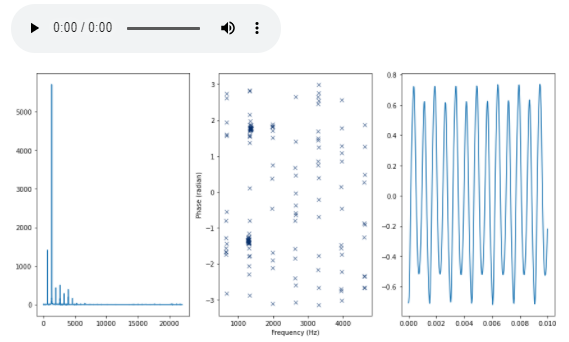
\includegraphics[width=\textwidth]{ex_3_spectrum.png}
                \caption{Результат вызова \texttt{plot-three} с \texttt{spectrum}}
                \label{fig:ex_3_spectrum}
            \end{figure}
            
            Теперь возмем функцию \texttt{zero-angle}, которая выдает результат, в котором \texttt{angle} = 0
            
\begin{lstlisting}[language=Python, caption= Функция \texttt{zero-angle}]
    def zero_angle(spectrum):
        res = spectrum.copy()
        res.hs = res.amps
        return res
\end{lstlisting} 
            
            После этого создадим \texttt{spectrum2}, вызвав \texttt{zero-angle} с \texttt{spectrum}:
            
\begin{lstlisting}[language=Python, caption= Вызов \texttt{plot-three} с \texttt{spectrum2}]
    spectrum2 = zero_angle(spectrum)
    plot_three(spectrum2, thresh=50)
\end{lstlisting} 
            
            \begin{figure}[H]
                \centering
                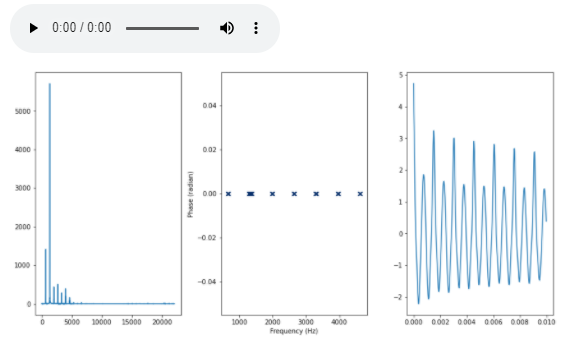
\includegraphics[width=\textwidth]{ex_3_spectrum2.png}
                \caption{Результат вызова \texttt{plot-three} с \texttt{spectrum2}}
                \label{fig:ex_3_spectrum2}
            \end{figure}
            
            Теперь возьмем функцию \texttt{rotate-angle}, которая выдает результат, в котором \texttt{angle} изменен на 1 радиан:
            
\begin{lstlisting}[language=Python, caption= Функция \texttt{rotate-angle}]
    def rotate_angle(spectrum, offset):
        res = spectrum.copy()
        res.hs *= np.exp(1j * offset)
        return res
\end{lstlisting} 
            
            После этого создадим \texttt{spectrum3}, вызвав \texttt{rotate-angle} с \texttt{spectrum}:
            
\begin{lstlisting}[language=Python, caption= Вызов \texttt{plot-three} с \texttt{spectrum3}]
    spectrum3 = rotate_angle(spectrum, 1)
    plot_three(spectrum3, thresh=50)
\end{lstlisting} 
            
            \begin{figure}[H]
                \centering
                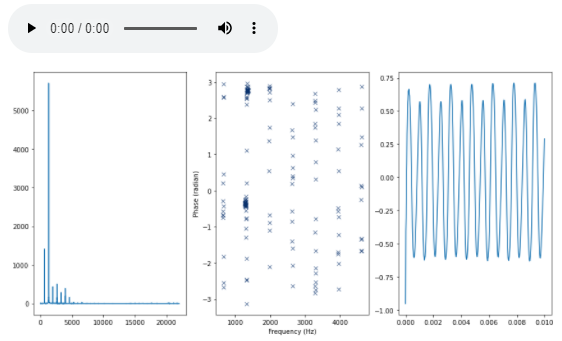
\includegraphics[width=\textwidth]{ex_3_spectrum3.png}
                \caption{Результат вызова \texttt{rotate-angle} с \texttt{spectrum3}}
                \label{fig:ex_3_spectrum3}
            \end{figure}
            
            Теперь возьмем функцию \texttt{random-angle}, которая выдает результат, в котором \texttt{angle} имеет рандомное значение:
            
\begin{lstlisting}[language=Python, caption= Функция \texttt{random-angle}]
    def random_angle(spectrum):
        res = spectrum.copy()
        angles = np.random.uniform(0, PI2, len(spectrum))
        res.hs *= np.exp(1j * angles)
        return res
\end{lstlisting} 
            
            После этого создадим \texttt{spectrum4}, вызвав \texttt{random-angle} с \texttt{spectrum}:
            
\begin{lstlisting}[language=Python, caption= Вызов \texttt{plot-three} с \texttt{spectrum4}]
    spectrum4 = random_angle(spectrum)
    plot_three(spectrum4, thresh=50)
\end{lstlisting} 
            
            \begin{figure}[H]
                \centering
                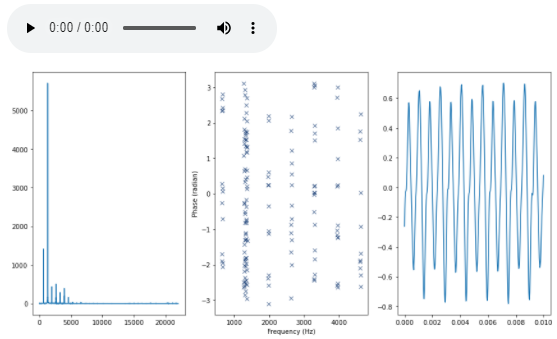
\includegraphics[width=\textwidth]{ex_3_spectrum4.png}
                \caption{Результат вызова \texttt{random-angle} с \texttt{spectrum4}}
                \label{fig:ex_3_spectrum4}
            \end{figure}
            
            В результате можно сказать, что рандомизация добавила глухой эффект, а также, что изменение \texttt{angle} почти не влияет на конечный сигнал.
            
    \newpage
        \section{Выводы}
             В результате выполнения данной лабораторной работы мы изучили, что такое ДКС, научились синтезировать ее и анализировать. Были проверены функции \texttt{analyze1} и \texttt{analyze2}, вычислили какая из этих функций работает быстрее и на сколько. Также создали функцию \texttt{make-dct-spectrogram} для сжатия звуковой дорожки и сразу ее проверили. Наконец, мы поработали с блокнотом \texttt{phase.ipynb}, пройдя по всем примерам с другим сегментом.
            
            
            
\end{document}
